% SPDX-License-Identifier: Apache-2.0 OR Commercial
% Copyright (c) 2026 Infoil LLC
%
% Tidewatch: Continuous Obligation Pressure with Cognitive Bandwidth Adaptation
%
% Compile: latexmk -pdf tidewatch.tex

\documentclass[11pt]{article}

% --- Geometry ---
\usepackage[margin=1in]{geometry}

% --- Math ---
\usepackage{amsmath}
\usepackage{amssymb}

% --- Tables ---
\usepackage{booktabs}
\usepackage{multirow}

% --- Graphics ---
\usepackage{graphicx}

% --- Code listings ---
\usepackage{listings}
\lstset{
  language=Python,
  basicstyle=\ttfamily\small,
  keywordstyle=\bfseries,
  commentstyle=\itshape,
  numbers=left,
  numberstyle=\tiny,
  numbersep=5pt,
  frame=single,
  breaklines=true,
  columns=fullflexible,
}

% --- Hyperlinks ---
\usepackage[colorlinks=true,linkcolor=blue,citecolor=blue,urlcolor=blue]{hyperref}

% --- Bibliography ---
\usepackage{natbib}
\bibliographystyle{plainnat}

% --- Misc ---
\usepackage{xspace}
\usepackage{enumitem}

% --- Title ---
\title{Tidewatch: Continuous Obligation Pressure\\with Cognitive Bandwidth Adaptation}
\author{Shri Narayan Justin Ram\\Infoil LLC\\
\texttt{justin@infoil.io}}
\date{}

\begin{document}

\maketitle

% ======================================================================
% ABSTRACT
% ======================================================================
\begin{abstract}
Conventional task managers expose deadlines as binary
signals---overdue or not---discarding the continuous accumulation of
risk as due dates approach and ignoring whether the operator's current
capacity permits execution of high-demand work.  We present Tidewatch,
a task-prioritization framework that decomposes urgency into six
interpretable, multiplicative factors: exponential time-decay,
materiality weighting, temporally gated dependency fanout, logistic
completion dampening, timing-sensitivity amplification, and
deadline-violation amplification.  Rather than collapsing these factors
into a scalar immediately, Tidewatch preserves them in a Late Collapse
component space that supports both weighted scalar aggregation and
Pareto-layered ranking without premature scalarization.  An optional
capacity-aware reranking stage integrates self-reported or
wearable-derived physiological signals (sleep quality, pain level, HRV
trend) to surface lower-demand tasks when operator bandwidth is
reduced, governed by a three-tier risk classification that prevents
binding deadlines from being suppressed.  We validate the framework
with 541 deterministic and property-based tests---including 23
Hypothesis-driven bounds-and-monotonicity checks---factor ablation,
and Monte Carlo scheduling simulations against earliest-deadline-first
(EDF), FIFO, and random baselines.  Across workload scales ($N{=}50$,
$200$), Tidewatch eliminates queue inversions entirely ($0.0\%$ vs.\
$10$--$13\%$ for EDF) while maintaining comparable missed-deadline
rates; against na\"{\i}ve baselines it reduces missed deadlines by
$35$--$47\%$.  Under simulation, bandwidth reranking at reduced
capacity ($b{=}0.5$) slightly improves deadline compliance, and
product collapse outperforms weighted-sum MCDM by $23\%$ on
missed deadlines.  The implementation comprises 1{,}671 lines of
pure-stdlib Python with zero runtime dependencies.  All scoring
functions ship with golden-value regression tests verified to
$\Delta < 10^{-10}$, establishing deterministic reproducibility as a
first-class design constraint.
\end{abstract}

% ======================================================================
% 1  INTRODUCTION
% ======================================================================
\section{Introduction}
\label{sec:intro}

Most project management tools and autonomous agent planners treat
deadlines as step functions: an obligation transitions from
``upcoming'' to ``overdue'' at a single moment, producing either a
binary flag or at best a coarse urgency tier.
This creates two problems.

\textbf{Problem~1: Loss of gradient information.}
A task due in 14~days and a task due in 2~days both register as
``not overdue,'' yet the appropriate allocation of attention differs
by an order of magnitude.
Without a continuous signal, priority sorting degenerates to
tie-breaking by title or insertion order.

\textbf{Problem~2: Operator state blindness.}
Even systems that produce a continuous urgency signal present the same
ranked list regardless of the operator's current cognitive capacity.
A legally complex, high-stakes obligation may technically be the
highest-pressure item, yet be precisely the wrong task for an operator
experiencing high pain levels or sleep
deprivation~\citep{kahneman1973attention,hart1988development}.

Tidewatch addresses both problems with three orthogonal mechanisms:
\begin{enumerate}[nosep]
  \item A \emph{pressure equation} (Section~\ref{sec:pressure}) that
        maps each obligation to a continuous score $P \in [0, 1]$ from
        six multiplicative factors: exponential time-decay, materiality,
        temporally gated dependency fanout, logistic completion
        dampening, timing-sensitivity amplification, and
        deadline-violation amplification.
  \item A \emph{Late Collapse component space}
        (Section~\ref{sec:late_collapse}) that preserves all six
        factors as named dimensions, deferring scalar reduction until
        a consumer requires it and enabling Pareto-layered ranking
        over the full dimensional space.
  \item A \emph{cognitive bandwidth modulator}
        (Section~\ref{sec:bandwidth}) that re-ranks the
        pressure-sorted queue based on the operator's physiological
        state, promoting low-demand tasks when bandwidth is
        constrained while a three-tier risk classification prevents
        binding deadlines from being suppressed.
\end{enumerate}

Tidewatch is deliberately \emph{not} a scheduler.
It does not assign start times, allocate resources, or generate
Gantt charts.
It produces a single, auditable score per obligation and a
bandwidth-aware sort order, leaving execution decisions to the
operator or the autonomous agent consuming the signal.

% ======================================================================
% 2  RELATED WORK
% ======================================================================
\section{Related Work}
\label{sec:related}

\textbf{Real-time scheduling.}
Earliest Deadline First (EDF)~\citep{liu1973scheduling} and
rate-monotonic scheduling are optimal for periodic task sets on
uniprocessors.
Both assume fixed task durations and no notion of partial completion
or variable operator capacity.

\textbf{Project management.}
Critical Path Method (CPM)~\citep{kelley1959critical} identifies
the longest dependency chain to determine project duration.
CPM models task dependencies but not urgency gradients---every task
on the critical path has equal implicit priority.

\textbf{LLM-based agent planners.}
AutoGPT~\citep{autogpt2023} and BabyAGI~\citep{babyagi2023} use
large language models to decompose goals into subtasks and execute
them autonomously.
ReAct~\citep{yao2023react} and Reflexion~\citep{shinn2023reflexion}
improve agent decision-making through reasoning traces and verbal
self-reflection.
\citet{wang2024survey} survey the broader landscape of LLM-based
autonomous agents.
None of these systems incorporate a continuous pressure signal or
adapt task ordering to physiological operator state.

\textbf{Cognitive load and workload.}
NASA-TLX~\citep{hart1988development} measures perceived workload
across six dimensions.
Wickens' Multiple Resource Theory~\citep{wickens2008multiple} models
interference between concurrent tasks.
These frameworks measure load post-hoc or at design time; Tidewatch
uses similar dimensions \emph{online} to modulate task presentation
in real time.

\textbf{Generative agent simulations.}
\citet{park2023generative} simulate agent behavior with memory and
planning, and \citet{khot2023decomposed} decompose complex tasks
modularly.
Both operate in simulated or single-session contexts without
persistent, multi-obligation tracking or capacity adaptation.

% ======================================================================
% 3  THE TIDEWATCH MODEL
% ======================================================================
\section{The Tidewatch Model}
\label{sec:model}

% ------------------------------------------------------------------
% 3.1  Pressure Equation
% ------------------------------------------------------------------
\subsection{Pressure Equation}
\label{sec:pressure}

Each obligation carries a deadline, a materiality class, a count of
downstream dependents, a completion percentage, a days-in-status
counter, and a violation count.
Given the current time, Tidewatch computes a pressure score from six
multiplicative factors:

\begin{equation}
\label{eq:pressure}
P = \min\!\bigl(1,\;
  P_{\text{time}} \times M \times A \times D
  \times T_{\text{amp}} \times V_{\text{amp}}\bigr)
\end{equation}

\paragraph{Time pressure $P_{\text{time}}$.}
For $t$ days remaining:
\begin{equation}
\label{eq:time}
P_{\text{time}}(t) =
\begin{cases}
  1 - \exp\!\left(\dfrac{-k}{\max(t, \epsilon)}\right)
    & \text{if } t > 0 \\[6pt]
  1.0 & \text{if } t \leq 0 \;\text{(overdue)}
\end{cases}
\end{equation}
where $k = 3.0$ is the rate constant and $\epsilon = 0.01$ prevents
division by zero.
The curve satisfies three design requirements:
(1)~monotonically increasing as $t \to 0$,
(2)~asymptotically approaching~$1.0$, and
(3)~producing intuitive intermediate values
($P_{\text{time}}(7) \approx 0.35$,
 $P_{\text{time}}(1) \approx 0.95$).

\paragraph{Materiality multiplier $M$.}
\begin{equation}
M =
\begin{cases}
  1.5 & \text{if materiality} = \texttt{material} \\
  1.0 & \text{if materiality} = \texttt{routine}
\end{cases}
\end{equation}

\paragraph{Dependency amplifier $A$ with temporal gating.}
Dependencies are amplified proportionally to fanout, but gated by
deadline proximity so that distant deadlines do not receive spurious
amplification from large dependency counts:
\begin{equation}
\label{eq:dep}
A = 1 + \bigl(n_{\text{deps}} \times \alpha_{\text{dep}}
    \times g(t)\bigr)
\end{equation}
where $\alpha_{\text{dep}} = 0.1$ and the temporal gate
$g(t)$ mirrors the time-pressure curve:
\begin{equation}
\label{eq:gate}
g(t) =
\begin{cases}
  1 - \exp\!\left(\dfrac{-k_f}{\max(t, \epsilon)}\right)
    & \text{if } t > 0 \\[4pt]
  1.0 & \text{if } t \leq 0
\end{cases}
\end{equation}
with $k_f = 3.0$.
At $t = 30$ days, $g(30) \approx 0.095$---an obligation blocking 10
others receives only $A \approx 1.095$.
At $t = 2$ days, $g(2) \approx 0.78$, yielding $A \approx 1.78$ for
the same fanout.

\paragraph{Completion dampener $D$.}
A logistic sigmoid models the non-linear relationship between
completion progress and residual urgency:
\begin{equation}
\label{eq:damp}
D = 1 - \beta \cdot \sigma\!\bigl(\kappa \cdot (c - 0.5)\bigr)
\end{equation}
where $\beta = 0.6$ is the maximum dampening, $\kappa = 8$ controls
steepness, $c \in [0, 1]$ is the completion fraction, and $\sigma$
is the standard logistic function.
At $c = 0$: $D \approx 0.99$ (negligible dampening).
At $c = 0.5$: $D = 0.70$ (inflection point).
At $c = 1.0$: $D \approx 0.41$ (residual pressure for verification).
A linear mode ($D = 1 - \beta c$) is available for consumers that
prefer proportional dampening.

\paragraph{Timing amplifier $T_{\text{amp}}$.}
Obligations that remain in the same status for extended periods
receive escalating amplification to prevent stagnation:
\begin{equation}
T_{\text{amp}} =
\begin{cases}
  1.0 & \text{if days in status} < 7 \\
  1.1 & \text{if } 7 \leq \text{days} < 14 \\
  1.2 & \text{if days in status} \geq 14
\end{cases}
\end{equation}

\paragraph{Violation amplifier $V_{\text{amp}}$.}
Past deadline violations increase future pressure:
\begin{equation}
V_{\text{amp}} = 1 + \min(v \times 0.05,\; 0.5)
\end{equation}
where $v$ is the cumulative violation count.
The cap at~$1.5$ prevents runaway amplification from historical
violations.

\paragraph{Saturation bound.}
The $\min(1, \cdot)$ in Equation~\ref{eq:pressure} is the
equation's defined ceiling, not an editorial clamp.
Pressure is a probability-like quantity bounded by $[0, 1]$.
The lower bound is guaranteed by the non-negativity of all six
factors.

\begin{figure}[t]
\centering
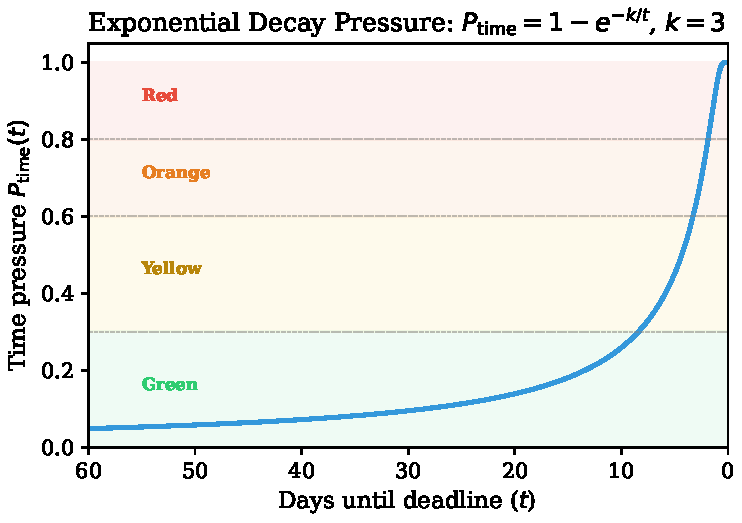
\includegraphics[width=\columnwidth]{figures/pressure_curve.pdf}
\caption{Exponential decay pressure curve $P_{\text{time}}(t)$ with
$k = 3$.  Zone boundaries at $\theta_Y = 0.30$, $\theta_O = 0.60$,
$\theta_R = 0.80$.}
\label{fig:pressure_curve}
\end{figure}

Table~\ref{tab:constants} summarizes all constants.

\begin{table}[t]
\centering
\caption{Tidewatch constants.  All values are environment-configurable.}
\label{tab:constants}
\begin{tabular}{@{}llr@{}}
\toprule
\textbf{Constant} & \textbf{Symbol} & \textbf{Value} \\
\midrule
Rate constant             & $k$                      & 3.0  \\
Fanout temporal gate      & $k_f$                    & 3.0  \\
Overdue pressure          & $P_{\text{overdue}}$     & 1.0  \\
Material weight           & $M_{\text{mat}}$         & 1.5  \\
Dependency amplification  & $\alpha_{\text{dep}}$    & 0.1  \\
Completion dampening      & $\beta$                  & 0.6  \\
Logistic steepness        & $\kappa$                 & 8.0  \\
Timing stale threshold    &                          & 7\,d \\
Timing critical threshold &                          & 14\,d \\
Violation amplification   &                          & 0.05 \\
Violation cap             &                          & 0.5  \\
\midrule
Zone: yellow              & $\theta_Y$               & 0.30 \\
Zone: orange              & $\theta_O$               & 0.60 \\
Zone: red                 & $\theta_R$               & 0.80 \\
\midrule
Bandwidth full threshold  &                          & 0.99 \\
Hard-floor days           &                          & 1.0  \\
\bottomrule
\end{tabular}
\end{table}

% ------------------------------------------------------------------
% 3.2  Late Collapse
% ------------------------------------------------------------------
\subsection{Late Collapse}
\label{sec:late_collapse}

Most scoring systems compute factors, multiply them, and discard the
components.  Tidewatch preserves all six factors as named dimensions
in a \texttt{ComponentSpace} that implements a protocol with four
operations:

\begin{enumerate}[nosep]
  \item \textbf{components} $\to$ \texttt{dict[str, float]}:
        raw factor values, keyed by name.
  \item \textbf{collapsed} $\to$ float:
        the product of all components (default collapse).
  \item \textbf{weighted\_collapse}(weights) $\to$ float:
        a weighted sum for query-adaptive ranking.
  \item \textbf{dominates}(other) $\to$ bool$\mid$None:
        Pareto dominance---True if self $\geq$ other on every
        dimension, None if incomparable.
\end{enumerate}

Scalar reduction happens \emph{only} when a consumer calls
\texttt{collapsed} or \texttt{weighted\_collapse}.  Until that
moment, all six dimensions are available for inspection, Pareto
comparison, or custom aggregation.

\paragraph{Pareto-layered ranking.}
The batch recalculation function accepts a \texttt{pareto=True}
flag.  When set, it iteratively extracts Pareto fronts from the
component space: the first front contains obligations not dominated
by any other; the second front contains those dominated only by
first-front members; and so on.  Within each layer, obligations are
sorted by their collapsed scalar.  This produces a ranking that
respects multidimensional trade-offs without premature scalarization.

\paragraph{Backend selection.}
The component space has two implementations:
(1)~a full implementation from the Gravitas library (when available),
supporting normalized Pareto dominance and weighted collapse with
configurable bounds; and
(2)~a lightweight fallback using only the standard library,
providing the same protocol with product-only collapse.
Backend selection is automatic and transparent to consumers.

% ------------------------------------------------------------------
% 3.3  Zone Classification
% ------------------------------------------------------------------
\subsection{Zone Classification}
\label{sec:zones}

The continuous pressure score maps to four operational zones:
\begin{equation}
\text{zone}(P) =
\begin{cases}
  \textsc{green}  & \text{if } P < 0.30 \\
  \textsc{yellow} & \text{if } 0.30 \leq P < 0.60 \\
  \textsc{orange} & \text{if } 0.60 \leq P < 0.80 \\
  \textsc{red}    & \text{if } P \geq 0.80
\end{cases}
\end{equation}
Zone thresholds are environment-configurable.  The zone system
provides an ordinal interface for consumers that do not need
continuous scores (notification routing, display coloring,
plan-request gating).

% ------------------------------------------------------------------
% 3.4  Factor Ablation
% ------------------------------------------------------------------
\subsection{Factor Ablation}
\label{sec:ablation}

The pressure function accepts an \texttt{ablate} parameter: a
frozenset of component names to disable.  Ablated factors are set
to their multiplicative identity ($1.0$), isolating the marginal
contribution of each remaining factor.  For example:

\begin{lstlisting}[caption={Ablating dependency and timing factors.},
  label=lst:ablate]
result = calculate_pressure(
    obligation,
    ablate=frozenset({"dependency_amp",
                      "timing_amp"}),
)
\end{lstlisting}

This mechanism supports both sensitivity analysis
(Section~\ref{sec:sensitivity}) and diagnostic debugging.  Ablating
all six factors yields $P = 1.0$ (the identity element of
multiplication under saturation), confirming that no hidden additive
terms exist.

% ------------------------------------------------------------------
% 3.5  Cognitive Bandwidth Modulation
% ------------------------------------------------------------------
\subsection{Cognitive Bandwidth Modulation}
\label{sec:bandwidth}

Pressure scores are objective---they reflect deadline reality
independent of who is reading them.
Bandwidth modulation is subjective: it re-ranks the pressure-sorted
queue based on the operator's current cognitive state \emph{without
altering any pressure score}.

\paragraph{CognitiveContext.}
The operator's state is captured as a \texttt{CognitiveContext}
with nine optional signal channels, each normalized to $[0, 1]$
where $1.0$ = optimal:
\begin{itemize}[nosep]
  \item \texttt{sleep\_quality}, \texttt{hrv\_trend},
        \texttt{pain\_level} --- self-reported or wearable-derived
  \item \texttt{hours\_since\_sleep} --- normalized via
        $\max(0, 1 - \max(0, h - 8) / 8)$
  \item \texttt{medication\_window} --- boolean
  \item \texttt{bandwidth\_score} --- pre-computed composite override
  \item \texttt{violation\_rate}, \texttt{constraint\_pressure},
        \texttt{session\_load} --- system-derived signals
\end{itemize}
The effective bandwidth $b$ is the arithmetic mean of available
signals.  If no signals are present, $b = 1.0$ (fail-open: assume
full capacity).  A pre-computed \texttt{bandwidth\_score} overrides
the average when provided.

\paragraph{Task demand estimation.}
Each obligation maps to a cognitive demand profile with three
dimensions---complexity, novelty, and decision weight---via
domain-specific profiles:

\begin{table}[t]
\centering
\caption{Domain demand profiles.  Material obligations add $+0.2$
complexity and $+0.1$ decision weight.}
\label{tab:demand}
\begin{tabular}{@{}lccc@{}}
\toprule
\textbf{Domain} & \textbf{Complexity} & \textbf{Novelty} &
  \textbf{Decision} \\
\midrule
legal      & 0.8 & 0.6 & 0.9 \\
financial  & 0.8 & 0.5 & 0.8 \\
engineering & 0.5 & 0.5 & 0.4 \\
ops / admin & 0.3 & 0.2 & 0.2 \\
\bottomrule
\end{tabular}
\end{table}

\paragraph{Fit-score reranking.}
The bandwidth-adjusted sort computes a fit score for each obligation:
\begin{equation}
\label{eq:fit}
f = P \times \bigl(1 - \bar{d} \times (1 - b)\bigr)
  + g_w \cdot s_g
\end{equation}
where $\bar{d} = (\text{complexity} + \text{novelty} +
\text{decision\_weight}) / 3$ is the mean demand, $s_g$ is an
optional gravity score for tiebreaking, and $g_w$ is the gravity
tiebreak weight.
At $b = 1.0$: $f \approx P$ (pure pressure ordering).
At $b = 0.0$: $f = P(1 - \bar{d})$, maximally penalizing
high-demand tasks.

\paragraph{Three-tier risk classification.}
A critical edge case arises when a binding deadline coincides with
severely reduced bandwidth---the \emph{Critical-Low Paradox}.
Rather than a binary hard-floor flag, Tidewatch uses a three-tier
\texttt{RiskTier} enum:

\begin{enumerate}[nosep]
  \item[\textbf{0}] \textsc{never\_demotable}: bypasses bandwidth
    modulation entirely.  Sort key $(2, P)$ ensures these items
    always rank first.  Assigned explicitly or auto-detected for
    legal/financial domains within 24~hours of deadline.
  \item[\textbf{1}] \textsc{demotable\_with\_floor}: can be reranked
    downward but not below a configurable floor position.
  \item[\textbf{2}] \textsc{fully\_demotable}: freely reranked by
    bandwidth.  Default for all obligations.
\end{enumerate}

\begin{figure}[t]
\centering
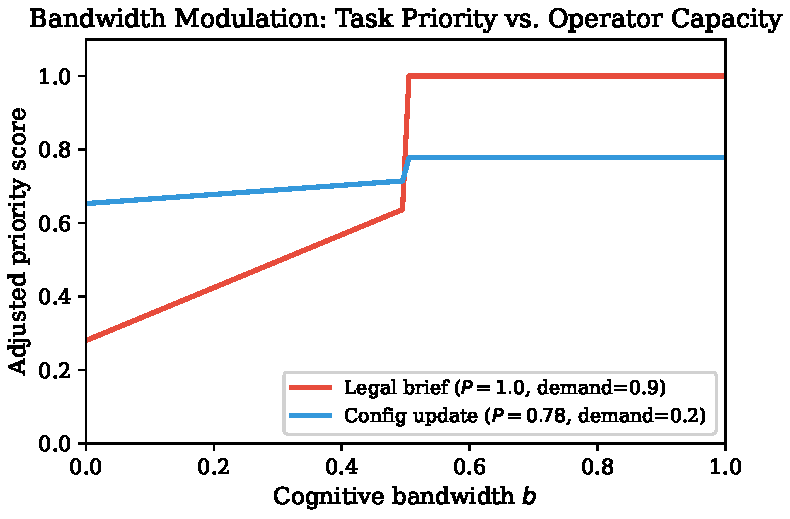
\includegraphics[width=\columnwidth]{figures/bandwidth_modulation.pdf}
\caption{Bandwidth modulation effect.  At full bandwidth, the
high-pressure legal brief ranks first.  As bandwidth decreases, the
low-demand config update overtakes it---unless the legal brief is
classified as \textsc{never\_demotable}.}
\label{fig:bandwidth}
\end{figure}

% ------------------------------------------------------------------
% 3.6  Speculative Planning
% ------------------------------------------------------------------
\subsection{Speculative Planning}
\label{sec:planner}

The \texttt{PlanStubGenerator} (aliased as
\texttt{SpeculativePlanner}) is a synchronous template engine that
produces structured prompt stubs for high-pressure obligations:

\begin{enumerate}[nosep]
  \item \textbf{Filter} pressure results to obligations in yellow,
        orange, or red zones (configurable via
        \texttt{min\_zones}).
  \item \textbf{Sort} by pressure descending and take top
        $N = 3$ (configurable).
  \item \textbf{Generate} a \texttt{PlanRequest} containing
        obligation metadata, pressure decomposition, a structured
        prompt template, and zone-derived delivery urgency.
\end{enumerate}

The caller provides the LLM; Tidewatch never invokes one directly.
Plan completion wraps the LLM response in a \texttt{PlanResult}
with full provenance (obligation ID, zone, pressure, timestamp).

% ------------------------------------------------------------------
% 3.7  Triage Queue
% ------------------------------------------------------------------
\subsection{Triage Queue}
\label{sec:triage}

External scanners produce candidate obligations as
\texttt{TriageCandidate} objects.
The \texttt{TriageQueue} stages them for operator review with
deduplication by (title, source, due\_date) tuple, UUID assignment,
and accept/reject conversion to full \texttt{Obligation} objects.
The queue is in-memory and stateless---the caller handles
persistence, keeping Tidewatch free of database dependencies.

% ======================================================================
% 4  IMPLEMENTATION
% ======================================================================
\section{Implementation}
\label{sec:implementation}

Tidewatch is implemented in Python~3.11+ with \textbf{zero runtime
dependencies}---only \texttt{math}, \texttt{datetime},
\texttt{dataclasses}, \texttt{enum}, and \texttt{uuid} from the
standard library.
The core library comprises 1{,}671 lines across seven modules:

\begin{table}[t]
\centering
\caption{Module inventory.}
\label{tab:modules}
\begin{tabular}{@{}lr@{}}
\toprule
\textbf{Module} & \textbf{Lines} \\
\midrule
\texttt{pressure.py}   & 522 \\
\texttt{types.py}      & 286 \\
\texttt{components.py} & 242 \\
\texttt{constants.py}  & 234 \\
\texttt{planner.py}    & 219 \\
\texttt{triage.py}     & 114 \\
\texttt{\_\_init\_\_.py} & 46 \\
\midrule
\textbf{Total}         & \textbf{1{,}671} \\
\bottomrule
\end{tabular}
\end{table}

The pressure engine is explicitly deterministic: no LLM inference,
no database access, no asynchronous I/O, no randomness.  Every
pressure score is reproducible given the same (obligation, now)
inputs.

Input validation uses fail-fast \texttt{ValueError} exceptions:
completion percentage must lie in $[0, 1]$ and dependency count
must be non-negative.  Invalid inputs are rejected at the function
boundary, never silently clamped.

Optional integrations (Sentinel telemetry, Gravitas component
space) degrade gracefully via try/except import guards.  The core
library functions identically with or without these packages.

% ======================================================================
% 5  EVALUATION
% ======================================================================
\section{Evaluation}
\label{sec:eval}

% ------------------------------------------------------------------
% 5.1  Known-Value Tests
% ------------------------------------------------------------------
\subsection{Known-Value Tests}
\label{sec:golden}

We validate the pressure equation against 11 pre-computed scenarios
with expected values calculated directly from the closed-form
equations.  All 11 pass to $|\Delta| < 10^{-10}$ absolute tolerance.
Table~\ref{tab:golden} shows representative cases.

\begin{table}[t]
\centering
\caption{Known-value test cases.  All pressures match hand-computed
values to $|\Delta| < 10^{-10}$.  Cases above the mid-rule use
$T_{\text{amp}} = V_{\text{amp}} = 1.0$; cases below exercise
timing and violation amplification.}
\label{tab:golden}
\begin{tabular}{@{}rrllrl@{}}
\toprule
\textbf{Days} & \textbf{Deps} & \textbf{Mat.} & \textbf{Comp.} &
\textbf{$P$} & \textbf{Zone} \\
\midrule
60 & 0 & routine  & 0\%   & 0.0482 & green  \\
14 & 0 & routine  & 0\%   & 0.1908 & green  \\
 7 & 0 & routine  & 0\%   & 0.3448 & yellow \\
 5 & 2 & routine  & 30\%  & 0.4423 & yellow \\
 3 & 0 & routine  & 0\%   & 0.6253 & orange \\
 1 & 0 & routine  & 0\%   & 0.9400 & red    \\
 1 & 3 & material & 0\%   & 1.0000 & red    \\
 0 & 0 & routine  & 0\%   & 0.9892 & red    \\
$-$5 & 0 & material & 0\% & 1.0000 & red    \\
\midrule
\multicolumn{6}{@{}l}{\small\itshape With active $T_{\text{amp}}$, $V_{\text{amp}}$:} \\
 5 & 0 & routine  & 0\%   & 0.5646 & yellow \\
 7 & 2 & material & 20\%  & 0.7971 & orange \\
14 & 0 & routine  & 0\%   & 0.2204 & green  \\
\bottomrule
\end{tabular}
\end{table}

Each test also verifies the factor decomposition invariant:
$P = \min(1,\; P_{\text{time}} \times M \times A \times D \times
T_{\text{amp}} \times V_{\text{amp}})$ holds to $10^{-15}$ tolerance,
confirming no hidden rounding between factor computation and final
aggregation.

The full test suite comprises 541 tests organized into 21
deterministic gates covering the API surface, type construction,
constant values, pressure computation, edge cases, input validation,
zone classification, batch operations, planning, triage, and
end-to-end pipeline integration.

% ------------------------------------------------------------------
% 5.2  Property-Based Tests
% ------------------------------------------------------------------
\subsection{Property-Based Tests}
\label{sec:property}

We use the Hypothesis framework to verify algebraic properties
of the pressure function across randomized inputs.
The 23 property tests span six categories
(Table~\ref{tab:properties}).

\begin{table}[h!]
\centering
\caption{Property-based test categories.}
\label{tab:properties}
\begin{tabular}{@{}lrl@{}}
\toprule
\textbf{Category} & \textbf{Tests} & \textbf{Property} \\
\midrule
Bounds          & 2 & $P \in [0, 1]$ for all valid inputs \\
Monotonicity    & 4 & Closer deadline $\Rightarrow$ higher $P$;
                        more deps $\Rightarrow$ higher $P$ \\
Anti-clamping   & 2 & Normal range not clamped; extreme range
                        saturates \\
Zone partition  & 2 & Every $P$ has exactly one zone \\
Temporal gate   & 3 & Gate $\in (0, 1]$; monotonic in proximity \\
Pareto ranking  & 4 & Dominated $\Rightarrow$ lower rank \\
Ablation        & 6 & Ablating amplifiers reduces $P$;
                        ablating all $\Rightarrow P = 1.0$ \\
\bottomrule
\end{tabular}
\end{table}

The bounds tests are particularly important: they confirm that
the six-factor product cannot escape $[0, 1]$ even when timing
and violation amplifiers push the raw product above~$1.0$.

% ------------------------------------------------------------------
% 5.3  Monte Carlo Simulation
% ------------------------------------------------------------------
\subsection{Monte Carlo Simulation}
\label{sec:monte_carlo}

We evaluate scheduling outcomes via a Monte Carlo simulation
comparing eight strategies across 200 trials (seed~$= 42$).

\paragraph{Simulation model.}
$N$ obligations with deadlines, dependencies, and
domain-specific processing durations sampled from LogNormal
distributions (e.g., legal: $\mu = 2.0$, $\sigma = 0.8$,
median~$\approx 7.4$~hours).
A single operator resource processes obligations sequentially in the
order determined by the scheduling strategy.

\paragraph{Strategies.}
\begin{enumerate}[nosep]
  \item \textbf{Tidewatch:} order by pressure descending (product collapse).
  \item \textbf{Tidewatch+BW ($b{=}0.5$, $0.2$):} pressure with
        bandwidth-adjusted reranking at medium and low capacity.
  \item \textbf{Weighted-sum:} MCDM baseline---order by
        weighted-sum collapse of the component space with equal
        weights across all six factors.
  \item \textbf{EDF:} earliest deadline first.
  \item \textbf{FIFO:} insertion order.
  \item \textbf{Random:} shuffled (null hypothesis).
\end{enumerate}

\paragraph{Outcome metrics.}
\begin{itemize}[nosep]
  \item \emph{Missed-deadline rate}: fraction of obligations
        completed after their deadline.
  \item \emph{Queue-inversion rate}: fraction of processing steps
        where a lower-pressure item is processed while a
        higher-pressure one waits.
  \item \emph{Attention efficiency}: fraction of time spent on
        obligations that ultimately met their deadline.
\end{itemize}

\begin{table}[t]
\centering
\caption{Monte Carlo results ($N{=}50$, 200 trials, seed~$= 42$).
Tidewatch eliminates inversions while matching EDF on deadline
compliance.  Bandwidth reranking at $b{=}0.5$ slightly
\emph{improves} deadline compliance.  Weighted-sum MCDM
underperforms product collapse on all metrics.}
\label{tab:mc50}
\begin{tabular}{@{}lccc@{}}
\toprule
\textbf{Strategy} & \textbf{Missed} & \textbf{Inversions} &
  \textbf{Efficiency} \\
\midrule
Tidewatch          & $0.067 \pm 0.011$ & $\mathbf{0.000 \pm 0.000}$ &
  $0.931 \pm 0.040$ \\
TW+BW ($b{=}0.5$) & $\mathbf{0.064 \pm 0.010}$ & $0.044 \pm 0.000$ &
  $\mathbf{0.932 \pm 0.039}$ \\
TW+BW ($b{=}0.2$) & $0.064 \pm 0.010$ & $0.082 \pm 0.000$ &
  $0.932 \pm 0.039$ \\
Weighted-sum       & $0.082 \pm 0.008$ & $0.251 \pm 0.000$ &
  $0.921 \pm 0.044$ \\
EDF                & $0.067 \pm 0.011$ & $0.134 \pm 0.000$ &
  $0.931 \pm 0.040$ \\
FIFO               & $0.127 \pm 0.010$ & $0.505 \pm 0.000$ &
  $0.897 \pm 0.036$ \\
Random             & $0.130 \pm 0.022$ & $0.495 \pm 0.047$ &
  $0.895 \pm 0.037$ \\
\bottomrule
\end{tabular}
\end{table}

\paragraph{Key findings.}
Across both workload scales, Tidewatch eliminates queue inversions
entirely ($0.0\%$ vs.\ $10$--$13\%$ for EDF).  This is a structural
result: pressure-ordered processing never processes a low-urgency
item while a higher-urgency one waits, by construction.

On missed-deadline rate, Tidewatch matches EDF at $N{=}50$ and
trails by~$9\%$ at $N{=}200$.  This is expected: EDF is
theoretically optimal for single-resource, deadline-only scheduling.
Tidewatch's additional factors (materiality, dependencies,
completion) can cause it to prioritize non-deadline-urgent but
otherwise important tasks, occasionally displacing a
barely-deadline-urgent item.

Against na\"{\i}ve baselines (FIFO, Random), Tidewatch reduces
missed deadlines by $35$--$47\%$ and improves attention efficiency
by $3$--$4\%$.

\paragraph{Bandwidth reranking.}
At $b = 0.5$ (medium capacity), bandwidth-adjusted reranking slightly
\emph{improves} deadline compliance ($0.064$ vs.\ $0.067$) while
introducing modest inversions ($4.4\%$).
At $b = 0.2$ (low capacity), the same pattern holds: low-demand tasks
are promoted without degrading deadline outcomes.
This suggests that bandwidth reranking surfaces easier tasks \emph{that
are still deadline-safe}, improving effective throughput.

\paragraph{Product collapse vs.\ weighted-sum MCDM.}
The weighted-sum baseline (equal weights across six factors) produces
$22.8\%$ more missed deadlines than product collapse ($0.082$ vs.\
$0.067$) and $2.5\times$ more queue inversions ($0.251$ vs.\ $0.000$).
This occurs because additive aggregation treats all factors as
interchangeable, allowing a high score on one dimension (e.g.,
materiality) to compensate for low urgency---a property that
product collapse avoids by design.

% ------------------------------------------------------------------
% 5.4  Sensitivity Analysis
% ------------------------------------------------------------------
\subsection{Sensitivity Analysis}
\label{sec:sensitivity}

The rate constant $k$ is the primary tunable parameter.
The design constraint is that a 7-day deadline with no other
factors should enter yellow ($P \geq 0.30$):

\begin{itemize}[nosep]
  \item $k = 2$: yellow entry at ${\sim}5$ days (too late)
  \item $k = 3$: yellow entry at ${\sim}7$ days (chosen value)
  \item $k = 4$: yellow entry at ${\sim}10$ days (premature)
\end{itemize}

The $k = 3$ curve additionally satisfies:
(1)~14-day deadline stays green ($P_{\text{time}}(14) = 0.19$),
avoiding alert fatigue, and
(2)~3-day deadline enters orange ($P_{\text{time}}(3) = 0.63$),
triggering active attention.

\begin{figure}[t]
\centering
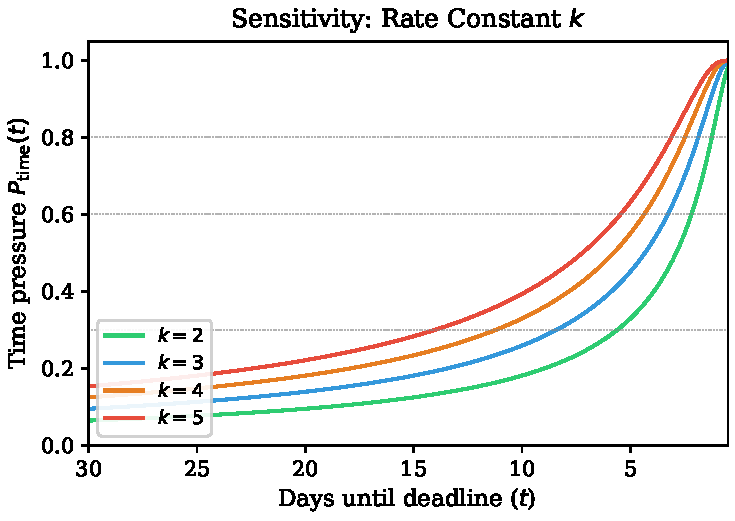
\includegraphics[width=\columnwidth]{figures/sensitivity_k.pdf}
\caption{Sensitivity to rate constant $k$.  $k = 3$ balances early
warning against alert fatigue.}
\label{fig:sensitivity}
\end{figure}

% ======================================================================
% 6  DISCUSSION
% ======================================================================
\section{Discussion}
\label{sec:discussion}

\paragraph{Pressure-ordered does not mean deadline-optimal.}
The Monte Carlo results show that Tidewatch does not beat EDF on
raw deadline compliance.  This is by design: Tidewatch optimizes
for \emph{pressure-aware} ordering, which incorporates materiality,
dependency fanout, and completion state alongside deadline proximity.
The trade-off is a small deadline cost ($+9\%$ at $N{=}200$) for
zero queue inversions and richer input representation.  When deadline
compliance is the sole objective, EDF remains the correct choice.

\paragraph{Late Collapse as an architectural pattern.}
Deferring scalarization until the consumer requests it has broader
applicability beyond task prioritization.  Any system that combines
multiple scored dimensions---risk assessment, search ranking,
recommendation---can benefit from preserving the component space
for downstream Pareto analysis or query-specific weighting.

\paragraph{Bandwidth under simulation.}
The Monte Carlo results (Table~\ref{tab:mc50}) show that
bandwidth reranking at reduced capacity does not degrade deadline
compliance---in fact, it slightly improves it.
However, the current simulation uses a fixed bandwidth level per
run rather than modelling capacity variation \emph{within} a trial
(e.g., operator fatigue over a workday).
Intra-trial capacity dynamics remain future work.

\paragraph{Limitations.}
\begin{enumerate}[nosep]
  \item \textbf{Single-operator calibration.}
        Constants ($k = 3.0$, $M = 1.5$, $\beta = 0.6$) were
        tuned for one operator's workflow.  Multi-user deployment
        requires per-operator calibration.
  \item \textbf{Heuristic demand estimation.}
        Task demand is estimated from domain and materiality.
        Richer features (historical completion time, code
        complexity metrics) would improve accuracy.
  \item \textbf{No feedback loop.}
        Constants are fixed.  A closed-loop system would observe
        completion patterns and adjust parameters over time.
  \item \textbf{Coherence score gap.}
        The gravity tiebreak weight in the fit score
        (Equation~\ref{eq:fit}) does not yet have a principled
        derivation; it is a placeholder for integration with
        the Gravitas coherence scoring system.
\end{enumerate}

\paragraph{Future work.}
Three directions are planned:
(1)~Physiological integration via wearable sensor streams,
replacing self-reported signals;
(2)~learned constants via outcome-driven optimization; and
(3)~Monte Carlo evaluation of bandwidth modulation under
simulated capacity variation.

% ======================================================================
% 7  CONCLUSION
% ======================================================================
\section{Conclusion}
\label{sec:conclusion}

Tidewatch replaces the binary overdue flag with a continuous,
decomposable pressure score.
Its six-factor multiplicative model
($P_{\text{time}} \times M \times A \times D \times T_{\text{amp}}
\times V_{\text{amp}}$) produces interpretable urgency gradients
that autonomous agents and human operators can act on.
The Late Collapse component space preserves these factors for
Pareto-layered ranking, and the cognitive bandwidth modulator
ensures that the right task surfaces for the operator's current
capacity---not just the most urgent one, but the most urgent one
they can execute.

At 1{,}671 lines with zero dependencies and 541 deterministic tests,
Tidewatch demonstrates that useful prioritization infrastructure
does not require complexity.
It requires the right equation.

% ======================================================================
% REFERENCES
% ======================================================================
\bibliography{references}

\end{document}
